\documentclass[a4paper,14pt]{article}
\usepackage[14pt]{extsizes}




\usepackage{cmap}					% поиск в PDF
\usepackage{mathtext} 				% русские буквы в формулах
\usepackage[T2A]{fontenc}			% кодировка
\usepackage[utf8]{inputenc}			% кодировка исходного текста
\usepackage[english,russian]{babel}	% локализация и переносы
\usepackage{ulem}                   % зачеркнутый текст
\usepackage{amssymb}			% пакет математики
\usepackage{float}
\usepackage{amsmath}
\usepackage{graphicx}
\DeclareGraphicsExtensions{.png}

%%% Страница
%\usepackage{extsizes} % Возможность сделать 14-й шрифт
\usepackage[left=1cm,right=1cm,top=1cm,bottom=1cm]{geometry} % Простой способ задавать поля
\pagestyle{empty}

\begin{document}


\begin{center}
ФЕДЕРАЛЬНОЕ ГОСУДАРСТВЕННОЕ ОБРАЗОВАТЕЛЬНОЕ БЮДЖЕТНОЕ УЧРЕЖДЕНИЕ ВЫСШЕГО ОБРАЗОВАНИЯ

    \textbf{«ФИНАНСОВЫЙ УНИВЕРСИТЕТ ПРИ ПРАВИТЕЛЬСТВЕ РОССИЙСКОЙ ФЕДЕРАЦИИ»}

Факультет информационных технологий и анализа больших данных

Департамент анализа данных и машинного обучения

\textit{
	\textbf{Дисциплина: «Теория вероятностей и математическая статистика»}}

\textit{Направление подготовки: 01.03.02 «Прикладная математика и информатика»}

\textit{Профиль: «Анализ данных и принятие решений в экономике и финансах»}

\textit{Форма обучения очная, учебный 2020/2021 год, 4 семестр}

\textbf{Билет 121}

\end{center}

\begin{enumerate}


\item


Дайте определение случайной величины, которая имеет $\chi ^{2}$-распределение с n степенями свободы.
Запишите плотность $\chi ^{2}$- распределения. Выведите формулы для математического ожидания $\mathbb{E}(X)$ и дисперсии $\mathbb{V}ar(X)$ $\chi ^{2}$-распределение с n степенями свободы. Найдите а) $\mathbb{P}(\chi _{20}^{2} > 10.9)$, где $\chi _{20}^{2}$–случайная величина, которая имеет $\chi ^{2}$– распределение с 20 степенями свободы; б) найдите 93\%
(верхнюю) точку $\chi _{0.93}^{2} (5)$ хи-квадрат распределения с 5 степенями свободы




$\mathbb{P}(\chi _{20}^{2} > 10.9) =  0.948775$; $\chi _{0.93}^{2} (5) = 1.34721$.


\item



Случайные величины $X$ и $Y$ независимы и имеют равномерное
распределение на отрезках $[0;3]$ и $[0;10]$ соответственно. Для случайной величины $Z=\frac{Y}{X}$ найдите: 
1) функцию распределения $F_Z(x)$;
2) плотность распределения $f_Z(x)$ и постройте график плотности;
3) вероятность $\P(3,\!263\leqslant Z\leqslant 5,\!35)$.




%\folder 2_53d23.png
1) Функция распределения $F_Z(x)$ имеет вид:
$
F_Z(x)=\left\{
\begin{array}{l}
0, x\leqslant 0;\\
\frac{3 x}{20}, 0\leqslant x\leqslant \frac{10}{3}\approx 3,\!333;\\
1 - \frac{5}{3 x}, x\geqslant\frac{10}{3};
\end{array}.
\right.
$
2) Плотность распределения $f_Z(x)$ имеет вид:
$
f_Z(x)=\left\{
\begin{array}{l}
0, x<0;\\
\frac{3}{20}, 0\leqslant x\leqslant \frac{10}{3}\approx 3,\!333;\\
\frac{5}{3 x^{2}}, x\geqslant\frac{10}{3};
\end{array}.
\right.
$


\begin{figure}[H]
    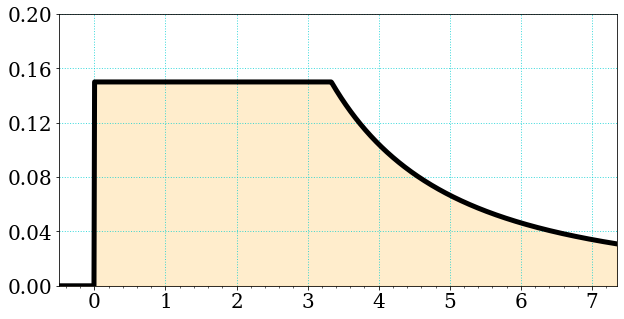
\includegraphics[width=0.9\textwidth]{2_53d23}
\end{figure}


3) вероятность равна:
$
\P(3,\!263\leqslant Z\leqslant 5,\!35)=
0,\!19897.
$


\item


(10) Известно, что доля возвратов по кредитам в банке имеет распределение $F(x) = x ^{\beta}, 0 \leqslant x \leqslant 1$.
Наблюдения показали, что в среднем она составляет $87,5\%$. Методом моментов оцените параметр $\beta$ и
вероятность того, что она опуститься ниже $53\%$




Найдём плотность рапределения как интеграл от ФР, а дальше всё и вовсе простою Ответ: $1174711139837$


\item


(10) В группе $\Omega$ учатся студенты:$\omega _{1}...\omega _{25}$ . Пусть $X$ и $Y$ – 100-балльные экзаменационные оценки по
математическому анализу и теории вероятностей. Оценки $\omega _{i}$ студента обозначаются: $x _{i} = X(\omega _{i})$ и $y _{i} = Y(\omega _{i})$, $i = 1...25$. Все оценки известны
$x _{0} = 33, y _{0} = 72$, $x _{1} = 94, y _{1} = 94$, $x _{2} = 91, y _{2} = 52$, $x _{3} = 47, y _{3} = 59$, $x _{4} = 53, y _{4} = 45$, $x _{5} = 96, y _{5} = 54$, $x _{6} = 60, y _{6} = 99$, $x _{7} = 70, y _{7} = 44$, $x _{8} = 50, y _{8} = 81$, $x _{9} = 57, y _{9} = 40$, $x _{10} = 99, y _{10} = 61$, $x _{11} = 94, y _{11} = 43$, $x _{12} = 85, y _{12} = 96$, $x _{13} = 30, y _{13} = 91$, $x _{14} = 57, y _{14} = 37$, $x _{15} = 42, y _{15} = 35$, $x _{16} = 84, y _{16} = 75$, $x _{17} = 96, y _{17} = 97$, $x _{18} = 69, y _{18} = 92$, $x _{19} = 91, y _{19} = 93$, $x _{20} = 45, y _{20} = 30$, $x _{21} = 35, y _{21} = 94$, $x _{22} = 83, y _{22} = 53$, $x _{23} = 53, y _{23} = 60$, $x _{24} = 36, y _{24} = 69$
Требуется
найти следующие условные эмпирические характеристики: 1) ковариацию $X$ и $Y$ при условии, что одновременно $X \geqslant 50$
 и $Y \geqslant 50$; 2) коэффициент корреляции $X$ и $Y$ при том же условии.




1) Ковариация = $-350.8333$
2) Коэффициент корреляции = $-1.2925$


\item


(10) Эмпирическое распределение признаков $X$ и $Y$ на генеральной совокупности $\Omega$ задано таблицей частот  
 
\begin{tabular}{ | c | c | c | c | }
\hline
 & $Y = 2$ & $Y = 4$ & $Y = 5$  \\ \hline
$X = 200$ & $1$ & $6$ & $23$\\ \hline
$X = 300$ & $13$ & $30$ & $27$\\
\hline
\end{tabular}

Из $\Omega$ случайным образом без возвращения извлекаются $13$ элементов. 
Пусть $\bar X$ и $\bar Y$ – средние значения признаков на выбранных элементах. 
Требуется найти: 1) математическое ожидание $\mathbb{E}(\bar Y)$; 2) стандартное отклонение $\sigma(\bar X)$ ; 
3) ковариацию $Cov(\bar X, \bar Y)$




1) математическое ожидание $\mathbb{E}(\bar Y)$: $4.22$ 
2) стандартное отклонение $\sigma(\bar X)$: $255.4769$
3) ковариацию $Cov(\bar X, \bar Y)$: $-1.2655$


\item

    
    	Юный аналитик Дарья использовала метод Монте-Карло для исследования Дискретного случайного вектора, описанного ниже.

        \begin{tabular}{|c|c|c|c|}
	\hline
	& X=$-3$ & X=$-2$ & X=$-1$ \\
	\hline
	Y = $2$ & $0.29$ & $0.298$  &  $0.234$ \\
	\hline
	Y = $3$ & $0.066$ & $0.03$ & $0.082$  \\
	\hline
\end{tabular}

    	Дарья получила, что E(Y|X + Y = 1) = $2.10982$.
    	Проверьте, можно ли доверять результату Дарьи аналитически. Сформулируйте определение метода Монте-Карло.
    


    
        $E(Y|X+Y=1) = \frac{\sum(P(X=1 - y_i, y=y_i) * y_i)}{\sum(P(X=1 - y_i, y=y_i)}$.

        Ответ: $2.10982$
    

\end{enumerate}

\begin{figure}[H]
	Подготовил
	\hfill
	
\includegraphics[width=2cm]{Prepared}
	П.Е. Рябов
\end{figure}


\begin{figure}[H]
	Утверждаю:\\
	Первый заместитель\\
	руководителя департамента\\
	Дата 01.06.2021
	\hfill
	
\includegraphics[width=2cm]{Approved}
	Феклин В.Г.
\end{figure}

\end{document}

